\documentclass[a4paper,11pt,portuguese]{article}
\usepackage{graphicx}
\usepackage{geometry}
\usepackage{hyperref}
\usepackage{float}
\usepackage{enumitem}
\usepackage{listings}
\usepackage[portuguese]{babel}

\geometry{margin=1in}


\begin{document}

%%% Identificação %%%

\author{
    Diogo Luís Henriques Costa - 50\% \\
    up201906731
    \and
    Francisco José Barbosa Marques Colino - 50\% \\
    up201905405
}
\title{FEUP -- Programação Funcional e em Lógica \large 2021/2022 \\ \large TP2 -- BreakthroughTanks\_1}
\date{\today}
\maketitle


%%% Instalação e execução %%%
\section{Instalação e execução}

% TODO
% o que dar include no sicstus e "play."


%%% Descrição do jogo %%%
\section{Descrição do jogo}

\href{https://boardgamegeek.com/boardgame/321224/breakthrough-tanks}{BreakthroughTanks}
é um jogo de tabuleiro de estratégia por turnos. É jogado por 2 jogadores oponentes, cada 
um controlando um conjunto de peças sobre um tabuleiro quadrangular, de dimensões pares, que podem variar
de 6x6 até 26x26. O objetivo do jogo é ser o primeiro a ter uma peça na linha mais distante, ou seja, a casa do oponente. 

\subsection{Peças}

\noindent Existem 3 tipos de peças:

\begin{enumerate}[topsep=4pt,itemsep=2pt]
    \item \textit{Medium tank}
    \item \textit{Heavy tank}
    \item \textit{Tank destroyer}
\end{enumerate}

\begin{figure}[H]
    \centering
    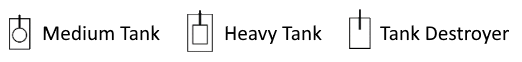
\includegraphics[width=0.5\textwidth]{imgs/pecas.png}
    \caption{Tipo de peças.}
    \label{fig:pecas}
\end{figure}

\noindent Num tabuleiro 8x8, cada jogador começa com 2 \textit{heavy tanks}, 4 \textit{tank destroyers}
e 10 \textit{medium tanks}. A sua disposição inicial no tabuleiro é a seguinte:

\begin{figure}[H]
    \centering
    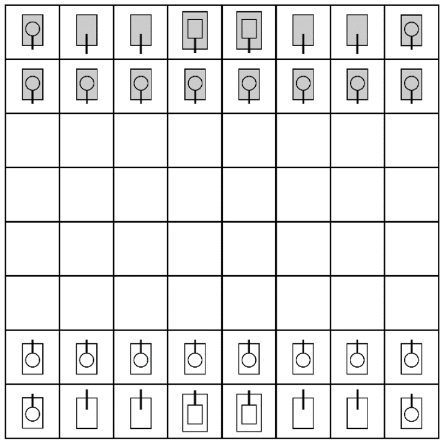
\includegraphics[width=0.25\textwidth]{imgs/board.png}
    \caption{Disposição inicial do tabuleiro.}
    \label{fig:board}
\end{figure}

\noindent Em todas as dimensões de tabuleiro, cada jogador fica com as linhas mais próximas de si completas com \textit{tanks}.
A 2ª linha mais próxima fica completa com \textit{medium tanks} e a linha mais próxima varia no número
de \textit{tank destroyers}, sendo que eles se posicionam em ambos os lados dos \textit{heavy tanks}.
Em todas as dimensões o posicionamento e quantidade (2) de \textit{heavy tanks} mantém-se.

\subsection{Movimentação simples}
Em cada turno uma peça faz uma movimentação simples ou executa uma captura. No caso 
da movimentação, esta é igual para todas as peças: uma unidade para a frente, ou uma 
unidade para uma das diagonais da frente.

\begin{figure}[H]
    \centering
    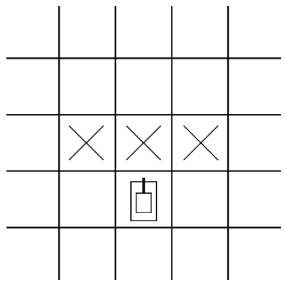
\includegraphics[width=0.2\textwidth]{imgs/movement.png}
    \caption{Movimentação.}
    \label{fig:movemente}
\end{figure}

\subsection{Captura}
Quando uma peça \textbf{A} captura uma peça inimiga \textbf{B}, a peça \textbf{B} é retirada do tabuleiro
e a peça \textbf{A} passa a ocupar o lugar anteriormente ocupado por \textbf{B}. 

\begin{enumerate}[topsep=4pt,itemsep=2pt]
    \item O \textit{Medium tank} captura da mesma forma que se move.
    \item O \textit{Heavy tank} captura 2 casas tanto para a frente 
    como nas diagonais da frente.
    \item O \textit{Tank destroyer} captura 2 casas para a frente.
\end{enumerate}

\noindent Neste jogo, o jogador não é obrigado a capturar caso seja possível.
Ele pode escolher capturar, ou mover a peça em causa de forma normal, ou até
mesmo mover outra peça.

\begin{figure}[H]
    \centering
    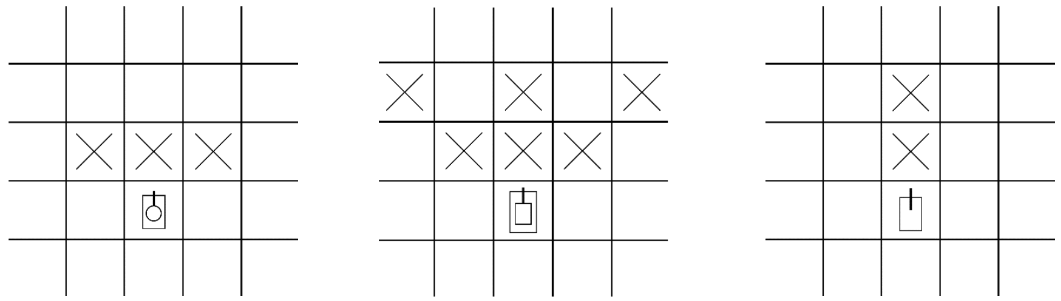
\includegraphics[width=0.5\textwidth]{imgs/capture.png}
    \caption{Captura de peças.}
    \label{fig:capture}
\end{figure}

\subsection{Fim do jogo}

O jogo acaba quando um jogador consegue chegar com uma peça sua à linha mais
afastada, ou seja, à linha mais próxima do oponente.
De notar que, caso um jogador fique sem peças, o seu adversário vence também o jogo.


%%% Lógica do jogo %%%
\section{Lógica do jogo}

    %%% Representação interna do estado do jogo %%%
    \subsection{Representação interna do estado do jogo}

    O estado do jogo, \textit{GameState}, é representado por: Turn-Board. Por sua vez, Turn pode ser ``top" ou ``bot"
    e Board é uma lista de listas de inteiros representando o tabuleiro.  

    \noindent O board é preenchido da seguinte forma:
    \begin{itemize}[topsep=4pt,itemsep=2pt]
        \item  0 -- Espaço vazio
        \item  1 -- \textit{Medium Tank} do \textit{bot player}
        \item  2 -- \textit{Heavy Tank} do \textit{bot player}
        \item  3 -- \textit{Tank destroyer} do \textit{bot player}
        \item -1 -- \textit{Medium Tank} do \textit{top player}
        \item -2 -- \textit{Heavy Tank} do \textit{top player}
        \item -3 -- \textit{Tank destroyer} do \textit{top player}
    \end{itemize}  

    \vspace{1em}
    Desta forma, cada tipo de \textit{tank}: \textit{medium tank, heavy tank, tank destroyer}, pode ser obtido
    recorrendo ao valor absoluto. Por outro lado, as peças de cada jogador distinguem-se pelo sinal: as peças do \textit{top player}
    têm representação interna negativa enquanto que as peças do \textit{bot player} têm representação positiva.

    \vspace{2em}
    \noindent Exemplos de estados de jogo:
    
    \subsubsection{Estado de jogo inicial, 8x8}
\begin{lstlisting}[language=prolog]
bot-[
        [ -1, -3, -3, -2, -2, -3, -3, -1],
        [ -1, -1, -1, -1, -1, -1, -1, -1],
        [  0,  0,  0,  0,  0,  0,  0,  0],
        [  0,  0,  0,  0,  0,  0,  0,  0],
        [  0,  0,  0,  0,  0,  0,  0,  0],
        [  0,  0,  0,  0,  0,  0,  0,  0],
        [  1,  1,  1,  1,  1,  1,  1,  1],
        [  1,  3,  3,  2,  2,  3,  3,  1]
    ]
\end{lstlisting}

    \noindent De modo a obter este estado, recore-se ao predicado
    $ initial\_state(+Size, -GameState) $ definido no ficheiro \textit{representation.pl}:
\begin{lstlisting}[language=prolog]
initial_state(Size, bot-Board):-
    between(6, 26, Size),
    even(Size),
    get_initial_board(Size, Board).
\end{lstlisting}


    \subsubsection{Estado de jogo intermédio, 8x8}
\begin{lstlisting}[language=prolog]
top-[
        [  0,  0,  0,  0,  0, -3, -3, -1],
        [  0,  0,  0,  0, -1, -1, -1, -1],
        [ -1,  2,  0,  0,  0,  0,  0,  0],
        [  0,  0,  0,  0, -2,  0,  0,  0],
        [  0,  0,  0,  0,  0,  0,  0,  0],
        [  0,  0,  0,  1,  0,  0,  0,  0],
        [  0,  0,  0,  0,  1,  1,  1,  1],
        [  1,  0,  0,  0,  0,  3,  3,  1]
]
\end{lstlisting}

    \subsubsection{Estado de jogo final, 8x8}
\begin{lstlisting}[language=prolog]
top-[
        [  2,  0,  0,  0,  0, -3, -3, -1],
        [  0,  0,  0,  0,  0, -1, -1, -1],
        [ -1,  0,  0, -1,  0,  0,  0,  0],
        [  0,  0,  0,  0,  0,  0,  0,  0],
        [  0,  0,  0,  1,  0,  0,  0,  0],
        [  0,  0,  0,  0,  0,  0,  0,  0],
        [  0,  0,  0,  0,  1,  1,  1,  1],
        [  1,  0,  0,  0,  0,  3,  3,  1]
    ]
\end{lstlisting}

    \noindent Neste caso o vencedor foi o \textit{bot player} dado que conseguiu
    alcançar a linha mais próxima do oponente com um dos seus \textit{tanks}.

    %%% Visualização do estado do jogo %%%
    \subsection{Visualização do estado do jogo}

    % TODO


    %%% Execução de jogadas %%%
    \subsection{Execução de jogadas}

    % TODO


    %%% Final de jogo %%%
    \subsection{Final de jogo}

    % TODO


    %%% Lista de jogadas válidas %%%
    \subsection{Lista de jogadas válidas}

    % TODO


    %%% Avaliação do Estado do Jogo %%%
    \subsection{Avaliação do Estado do Jogo}

    % TODO


    %%% Jogada do Computador %%%
    \subsection{Jogada do Computador}

    % TODO


%%% Conclusões %%%
\section{Conclusões}

% TODO


%%% Bibliografia %%%
\section{Bibliografia}

%% TODO embelezar
https://boardgamegeek.com/boardgame/321224/breakthrough-tanks
% TODO if necessary


\end{document}
